\documentclass[a4paper,man,natbib,floatsintext,donotrepeattitle]{apa6}

\usepackage[english]{babel}
\usepackage[utf8x]{inputenc}
\usepackage{amsmath}
\usepackage{graphicx}
\usepackage[colorinlistoftodos]{todonotes}
\usepackage{xcolor}
\usepackage[draft,inline,nomargin,index]{fixme}
\usepackage{hyperref}
\usepackage{verbatim}
\usepackage{nameref}
\usepackage{booktabs}
\usepackage{lineno}
\usepackage{amsfonts}
\usepackage{booktabs}
\usepackage{siunitx}
\linenumbers

\fxsetup{theme=color,mode=multiuser}
\FXRegisterAuthor{ab}{sab}{\color{blue}Amelie} % abnote{} with text inside to edit
\FXRegisterAuthor{bb}{sbb}{\color{purple}Brice} % bbnote{} with text inside to edit
\FXRegisterAuthor{ln}{sln}{\color{violet}Lad} % lnnote{} with text inside to edit

%\title{Blinding as a Necessary Precaution Against Experimenter Biases During Sequential Bayes Factor: A commentary on \cite{schonbrodt_sequential_2017}}

%\title{On the importance of blinding during sequential testing procedures: A commentary on \cite{schonbrodt_sequential_2017}}

%\title{"Efficient" yes, but only if you blind yourself: A commentary on \cite{schonbrodt_sequential_2017}}

%\title{"Efficient", but blind yourself as a precaution: A commentary on \cite{schonbrodt_sequential_2017}}

%\title{Blinding as a Precaution Against Experimenter Biases During Sequential Testing: A commentary on \cite{schonbrodt_sequential_2017}}

%\title{Triple Blinding for Sequential Testing: A commentary on \cite{schonbrodt_sequential_2017}}
\title{Automation in Sequential Testing: A commentary on \cite{schonbrodt_sequential_2017}}

\shorttitle{Blind Bayes Factor}
\threeauthors{Amélie Bret}{Brice Beffara}{Ladislas Nalborczyk}
\threeaffiliations{Univ. Grenoble Alpes, CNRS, LPNC, 38000 Grenoble, France \\ Psychological Science Research Institute, Catholic University of Louvain, Belgium \\ The Walden III Slowpen Science Laboratory, France}{The Walden III Slowpen Science Laboratory, Villeurbanne, France \\ 
Univ Lyon, ENTPE, LGCB, F-69518 Vaulx-en-Velin, France}{Univ. Grenoble Alpes, CNRS, LPNC, 38000 Grenoble, France \\ Department of Experimental Clinical and Health Psychology, Ghent University \\ The Walden III Slowpen Science Laboratory, France}

\abstract{We discuss the use of the Sequential Bayes Factor (SBF) procedure as introduced by \cite{schonbrodt_sequential_2017} when confronted to real world data. Contrary to simulated data, real world data can be complicated to handle. Several choices have to be made before fitting a model to ensure that subsequent model comparison is sensible. The SBF procedure is expected to inform us about the adequate sample size to reach a conclusion, based on accumulating data. Accordingly, we suggest that one should also prepare data in a sequential way before actually computing a Bayes Factor. \lnnote{In other words, a good model set is a prerequisite for sensible model comparison.} We propose a full automation procedure, in line with the preregistration philosophy, allowing triple-blinding of analyses. We provide recommendations on how to implement this without additional costs, while taking into account the specificity of the sequential testing situation.}

\keywords{Sequential Bayes Factor, sequential testing, automation, preregistration, blind analyses}

% re-enabling section numbering (disabled by the apa6.csl)
% \setcounter{secnumdepth}{3}

\begin{document}

% defining a new command for counting words
\newcommand{\quickwordcount}{%
  \immediate\write18{texcount -1 -sum -merge \jobname.tex > \jobname-words.sum }%
  \input{\jobname-words.sum}words%
}

\maketitle

Wordcount: This document contains \textbf{\quickwordcount}.

\newpage

%\tableofcontents % provisoire, juste pour se repérer entre nous
%\newpage

%%%%%%%%%%%%%%%%%%%%%%%%%%%%%%%%%%%%%%%%
% début du comment
%%%%%%%%%%%%%%%%%%%%%%%%%%%%%

\newpage

\section{Introduction}

\cite{edwards_ward_bayesian_1963} state, "the rules governing when data collection stops are irrelevant to data interpretation. It is entirely appropriate to collect data until a point has been proven or disproven, or until the data collector runs out of time, money, or patience". However, this practice has severe pitfalls in the classical NHST paradigm, as it dramatically increases Type I error rates, which therefore need to be controlled \citep{lakens_performing_2014}. % \cite{schonbrodt_sequential_2017} say: "Of course, one can calculate statistics during data collection, but the results of these tests must not have any influence on optionally stopping data collection."

In their paper, \cite{schonbrodt_sequential_2017} present an alternative to NHST with a priori power analysis (NHST-PA). They introduce the \textit{Sequential Bayes Factor} (SBF) procedure that allows to collect data iteratively, until a predefined threshold is reached, while not suffering from the pitfalls associated with NHST-PA. Testing mean differences between two independent groups, they show that the SBF design typically needs 50\% to 70\% smaller samples to reach a conclusion about the presence of an effect, as compared with optimal NHST-PA (where \textit{optimal} stands for an idealized situation in which the a priori targeted effect would be exactly equal to the population effect size), while having similar long-term error rates.

However, while the procedure described in \cite{schonbrodt_sequential_2017} offers an attractive perspective on data collection and while we generally agree with most of their recommendations, we draw attention about precautions that need to be undertaken in order to preserve the long-term rates of wrong inference they provide. One major concern is that dealing with real-world data, we know that many analysis choices can be made before model comparison. Depending on the type of data, researchers can have to deal with signal processing, outliers rejection, checking assumptions of the model, and other potential prerequisites, required before actually comparing two models (i.e., before computing a Bayes Factor). Dealing with these choices without influencing optionally stopping data collection entails that the data analyst should not interact with data during data collection. Hence all these decisions have to be made and implemented before data collection. To this end, we propose a full automation sequential procedure from data extraction to model comparison, embedded in the preregistration philosophy, with byproduct methodological advantages.

%We argue that such interim analysis (including visual inspections of the data) might have an influence on future data collection through overlooked experimenter effects, thus biasing the expected results of sequential testing procedures (both Bayesian and frequentist). While the procedure described in \cite{schonbrodt_sequential_2017} offers an attractive perspective on data collection and while we generally agree with most of their recommendations, we draw attention about precautions that need to be undertaken in order to preserve the long-terms rates of wrong inferences they provide. One major concern is that the person who runs the experiment and the person who analyses the data are usually the same person. As noted by \cite{wicherts_degrees_2016}, in the psychological field, "the analyses are typically conducted by a person who is not only aware of the hypotheses, but also benefits directly from corroborating them". Thus, failures of blinding procedures are listed among the 34 researchers degrees of freedom identified by \cite{wicherts_degrees_2016}. In the current commentary we highlight the particular dramatic consequences of blinding failures in the context of sequential testing, and suggest a new way to combine triple blinding with sequential testing, taking into account the specificities of such procedures.

\section{Intrapersonal biases in SBF procedure}

When a data analyst has expectations about what should be observed, data analysis is likely to be biased by these expectations through confirmation (favoring an hypothesis) or disconfirmation (stronger skepticism toward data against the hypothesis than toward data corroborating the hypothesis) biases \citep{lilienfeld_blind_2017}.
When sequentially computing a Bayes Factor (BF), we are faced with many choices about how to deal with new incoming data. Based on previous studies, we might have expectations about the range of plausible values, particular methods to process physiological signals, the need for recoding or transforming data, or the distribution of residuals, or many others. We propose that these decisions should be made before starting the SBF procedure.

The SBF procedure has been validated based on simulated data \citep{schonbrodt_sequential_2017}. However, noise and irregularities in simulated data can only come from sampling variability, and not from practical problems encountered during empirical data collection (e.g., participant or experimenter errors). What we want when dealing with real world data is to get as close as possible to the ideal case of simulated data. In order for the Bayes Factor to be a reliable stopping criterion, it has to be computed on relevant/reliable data. What we call relevant data can be decided relatively to the type of study, and justified by the existing literature as much as possible. What should not be done is changing the criterion and methods for data preparation based on some states of the SBF procedure. This implies that i) the researcher is well aware of the literature of interest and deeply thought about how to analyze data before collecting it, ii) the researcher knows how data behave by manipulating data from very similar previous experiments or pre-tests, iii) the researcher is able to implement a procedure of data preparation for model computation before seeing new data. These three points might seem trivial but are even more important for sequential testing than classical procedures in order to avoid intermediate influences in data preparation based on known interim BF.

When carefully decided, we propose that all these treatments should be automated and performed at each step of the sequential testing procedure. This way,  data preparation and verification such as (for instance) outliers' detection, data transformation or model assumption checks, would be done in an incremental manner, with the entire dataset always reconsidered - including former outliers -, so that this process would follow the progressive incorporation of new observations (i.e., such a procedure should be able to take into account that an extreme observation at time \textit{t} might not be extreme anymore at time \textit{t+n}). The fact that this iterative procedure is automated should prevent the data analyst from classical traps during data manipulation. Theses traps could have much more important consequences in SBF in comparison to traditional procedures due to the incremental nature of evidence accumulation. Besides, this idea fits well with the open science philosophy and with preregistration practices. Indeed, we propose that these steps would be programmed and coded on the basis of preregistered choices, before starting to collect data. Preregistered automated data analysis would therefore ensure the error rates of empirical SBF procedures to be similar to the long-term error rates provided by \cite{schonbrodt_sequential_2017} using simulation, and explicitly fulfill the requirements of transparent and reproducible science. \par

With full automation of data preparation during the SBF procedure, we aim to bring it closer to the recommendations of \cite{schonbrodt_sequential_2017} by reducing possible intermediate influences risked to be encountered both at the data collection and data analysis levels. Besides these considerations about data analysis, we can anticipate some basic mechanisms of intermediate influence on data collection, avoidable with full automated SBF.

\section{Interpersonal biases in SBF procedure}

When an experimenter has expectations about what should be observed, data collection is likely to be biased by these expectations \citep{orne_social_1962,rosenthal_social_1963,rosenthal_experimenter_1964,rosenthal_interpersonal_1978,zoble_interaction_1969,klein_low_2012,gilder_role_2018}.

Double (participant and experimenter) blind designs are expected to minimize expectancy effects \citep{klein_low_2012,gilder_role_2018}. When the experimenter cannot be blind, expectancy effects are clearly expected. If "experimenter bias is important to consider when
performing a study under normal circumstances", it "becomes even more important to consider
when the experimenter has performed an interim analysis" \cite{lakens_performing_2014}. \par

What is the specific status of sequential testing concerning analyst and observer expectancy effects ? Expectancy effects arise when one has prior beliefs and/or motivations about the issue of an experiment and involuntarily (we assume scientific honesty) influences the results on the basis of these prior beliefs and motivations. The confidence toward an hypothesis can be influenced by previous results from the literature, naive representations about the studied phenomenon, and all other sources of information. All these sources of information may deal with the studied phenomenon but rarely with the ongoing study specifically, as a consequence, the confidence about an hypothesis is always subject to uncertainty. When performing sequential testing, one has a direct access to accumulation of evidence concerning the ongoing study. Hence, the prior information accumulated from SBF is far more certain than information gathered form previous studies or naive representations. Hence, the risk to fall into an "evidence confirmation loop" is increased. In the previous section, we proposed that tis risk applies to confirmation and disconfirmation biases (data analysis) where the intrapersonal bias of data evaluation can inflate with accumulated evidence. We also propose that observer expectancy effects during data collection, where the interpersonal bias of experimenter-participant interaction can inflate with accumulated evidence. 

Obviously, It is very hard to obtain robust results concerning the effect size of analyst and observer expectancy effects. This "meta-science" problem is complicated because these biases can apply at all the levels as one experiment is included in another. For instance \cite{barber_expecting_1978} suggests that expectancy biases can occur in the expectancy bias research. It can also be difficult to collect large observation samples by experimental conditions \citep[e.g.,][]{zoble_interaction_1969} Even if a recent massive work showed that it is not impossible \citep {gilder_role_2018}. Thus, we can only draw attention to these effects as a potential risk to consider rather than as clearly quantified danger to avoid. \par

When classical double (participant and experimenter) blind designs are not practicable, interpersonal bias seem obvious. In a double blind design, the existence of an interpersonal bias is probably more questionable. How could knowledge about the data influence the issue of the experiment ? It is possible that the experimenter's verbal and non-verbal motor cues impact the participant's behavior \citep{zoble_interaction_1969}. In a double-blind design, the experimenter cannot influence the participant's responses on the basis of the experimental condition knowledge. However, the (de)motivation and the disappointment/satisfaction of seeing the preferred hypothesis contradicted/confirmed by the sequential testing procedure can possibly influence the participant. We cannot exclude that the confidence in an hypothesis can interact with experimental conditions and impacts the issue of the experiment in one way or another. Because the experimenter is not aware of the experimental condition of the participants, s·he can influence them only uniformly. This means that the behavior of the experimenter can potentially change the baseline of a parameter in all participants. We cannot exclude for sure that the effect of the experimental manipulation can be biased by this baseline change. More generally, "contextual variables, such as experimenters’ expectations, are a source of error that obscures the process of interest" \citep{klein_low_2012}.\par

To our knowledge, expectancy biases have never been reported when the experimenter was blind to the experimental condition. However, blinding the experimenter from interim analysis should be more certainly recommended \citep{lakens_performing_2014} when blinding experimental conditions is not practicable. We suggest that blinding analysis can also be considered as a precaution even when the experimenter is blind.

In the following, we describe hypothetical observable consequences of such biases on the SBF procedure. Importantly, expectation bias can emerge in all combinations of a priori expectations and population effect size (see Table \ref{tab:pred}).

%\begin{figure}[H]
%  \caption{Overview of the SBF procedure and illustration of potential biases when the experimenter and the data analyst are the same person.}
%  \centering
%  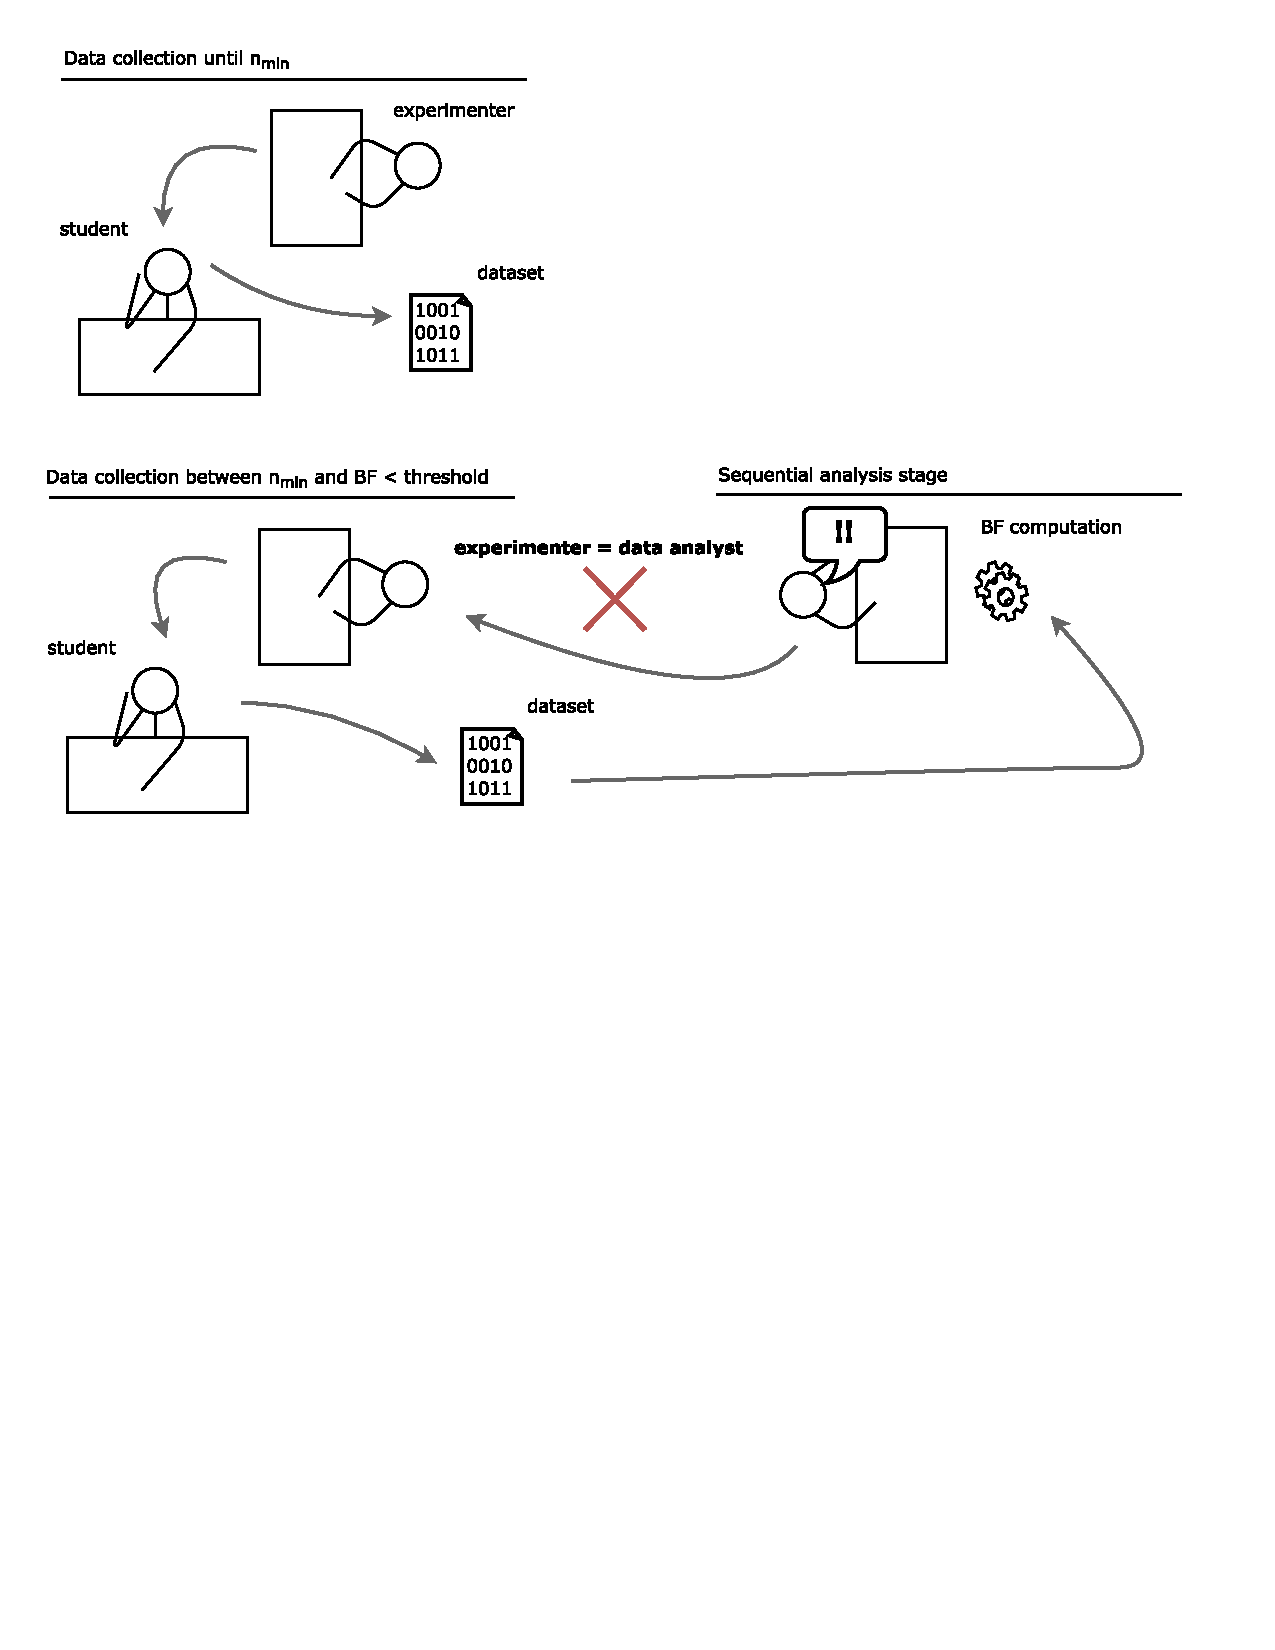
\includegraphics[width=0.8\textwidth]{figures/bias_diag.pdf}
%  \label{fig:diag1}
%\end{figure}

%\vline

%\begin{table}
%  \centering
%	\begin{tabular}{SSSS} \toprule
%     & \textbf{True} & & \\ 
%    \textit{Expected} & {effect} & \textit{H0} & \textit{H1} \\ \midrule
%     & \textbf{H0} & {+H0} & {-H0} \\
%     & \textbf{H1} & {-H1} & {+H1} \\ \bottomrule 
%	\end{tabular}
%    \caption{Possible interactions between true and expected effect on its %observation. + = accelerate and - = decelerate convergence.} %\label{tab:hexp}
%\end{table}
%\par

\vspace{5mm}

\begin{table}[H]
\centering
\caption{Possible interactions between population effect size and a priori beliefs during a sequential testing procedure. Congruent observations are expected to increase the speed of threshold reaching (H0+ and H1+), while incongruent observations are expected to slow down the process (H0- and H1-), and to increase the number of false alarms.}
\label{tab:pred}
\resizebox{\textwidth}{!}{%
\begin{tabular}{@{}ccc@{}}
\toprule
 & \begin{tabular}[c]{@{}c@{}}There is no difference in the population\\ (H0, $\delta = 0$)\end{tabular} & \begin{tabular}[c]{@{}c@{}}There is a difference in the population\\ (H1, e.g., $\delta = 0.5$)\end{tabular} \\ \midrule
Researcher 1, believes in H0 & H0+ (congruent) & H0- (incongruent) \\
Researcher 2, believes in H1 & H1- (incongruent) & H1+ (congruent) \\ \bottomrule
\end{tabular}%
}
\end{table}

Again, evidence is insufficient to conclude that analyst and observer expectancy effects are absolutely necessary to take into account. If the cost of reducing the bias was high, we could be skeptical about considering it, knowing its uncertain benefits. However, as we will suggest in the next sections, very easy to implement and costless methods can be applied to overcome these biases. Hence, even with low certainty about the risks, it is worthwhile to limit it all the same.

These biases can wear a multitude of forms as it is a function of the researcher \textit{a-priori} expectancies and of the population effect size. Moreover, we focus here on the simplest case in which the expectancies of the researcher remain constant throughout the sequential testing procedure. Although probably non realistic, this setting serves illustrative purposes. Figure \ref{fig:pred} illustrates our predictions concerning the biased evolution of Bayes Factor during sequential testing, according to the four situations presented in Table \ref{tab:pred}. The main message is that congruent situations (i.e., H0+ and H1+) would make the predefined boundary faster to reach (i.e., the sample size at which the boundary is hit would be lower than usually) and would lower error rates, while incongruent situations (i.e., H0- and H1-) would slow down this process and increase error rates.

\begin{figure}[H]
  \caption{Predicted consequences on the result of a SBF procedure with a fixed boundary of BF10 = 6 (or BF10 = 1/6), for a given Cohen's d of 0.5 (hereafter, "H1") or of 0 (hereafter "H0"), and according to the \emph{a priori} researcher expectancies.}
  \centering
  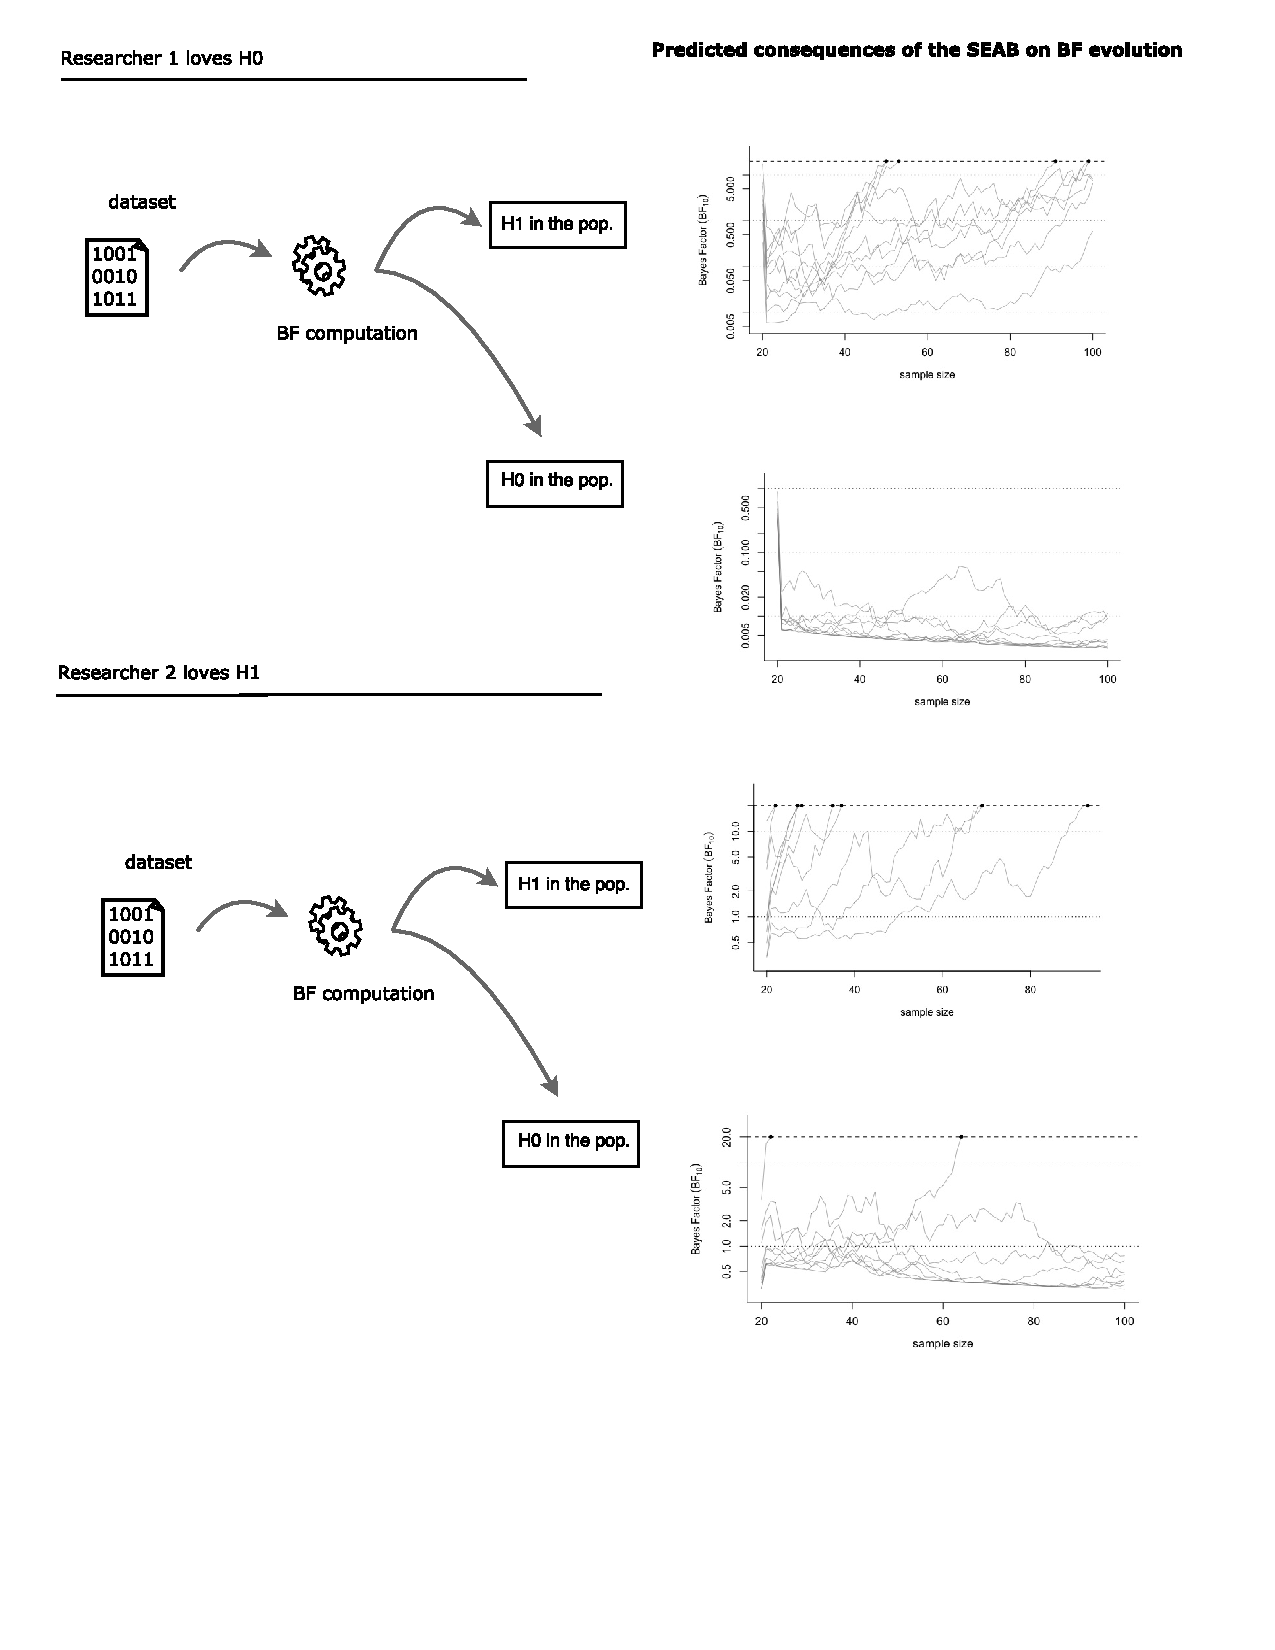
\includegraphics[width=0.8\textwidth]{figures/BFF_predictions.pdf}
  \label{fig:pred}
\end{figure}

Having presented the mechanisms through which we expect the knowledge of previous data to influence the data collection process, and illustrated the predicted consequences of these biases on the evolution of sequentially computed Bayes Factors, we focus on the next section on how to prevent this to happen. We suggest two ways of implementing triple blinding as a precaution against experimenter biases during sequential testing, and present the concepts of an automated procedure that would ensure objectivity.

\section{Strengths and weaknesses of automation as compared to classical blinding.}

\subsection{Solution 1: one analyst, one experimenter}

%Hence, we suggest doing triple blinding is which participants, experimenter and data analyst are not aware of the experimental informations (conditions, hypothesis...)

Double (participant and experimenter) blinding advantages is now well documented \citep{schulz_blinding_2002}. If this procedure can minimize the problem of experimenter effect (in the SBF procedure), it is not always practicable. Although experimenter blinding procedures have became a gold standard in many psychological fields, much less attention has been dedicated to analysis blinding. In the SBF procedure analysis blinding can take two different meanings. The classical meaning is a procedure ensuring that the person who analyses the data is blind to hypotheses (minimizing intra-personal biases). The meaning probably more specific to sequential testing is a procedure ensuring that the experimenter is blinded to data analysis (minimizing interpersonal biases). Analysis blinding has first been applied with great success in clinical trials, where \textit{triple} refers to the fact that the committee who assess the results of a trial is blind to the hypothesis. Applied to data analysis, triple blinding refers to a situation in which data analysis is performed by an individual who is not aware of the hypotheses and thus, who has not particular interest in corroborating or disproving it \citep{miller_blind_2011}. This practice, while not largely spread in psychology, would be a remedy for many of the biases identified in \cite{wicherts_degrees_2016}. However, we understand that it is a luxury possibility and it is not easy to apply, mostly due to materials and time constrains.

\subsection{Solution 2: one analyst-experimenter, "software-blinded"}

Another solution is to automate analysis blinding, so that the data analyst and the experimenter (who can be the same person) are blind to Bayes Factors computed on previous sets of observations. To illustrate this idea, we wrote a short function allowing to run a SBF for two-independent groups comparison. The user can set the \texttt{blind} argument to \texttt{TRUE}, and be completely blind to the results of the SBF procedure. The only output is a sentence that either indicates to "continue" or to "stop" the recruitment, considering an a-priori defined threshold (see \nameref{sec:supp} for code details). The main advantage of this solution is that it's a costless and ready-to-use solution.

Moreover, we also implemented  for a more complete treatment of the biases that can emerge during sequential testing, we suggest to combine the automated proposed in the first part of this comment with triple blind. We used... (https://osf.io/apidb/)...

To sum up, we suggest to combine the automated preprocessing steps proposed in the first part of this comment, with triple blind, to ensure objectivity during sequential testing.

%\texttt{seqBF} function, written by Félix Schönbrodt \& Richard Morey (available \href{https://raw.githubusercontent.com/richarddmorey/BayesFactorExtras/master/BayesFactorExtras/R/seqBF.R}{here}),

%\subsection{Experimental demonstration}
%After Rosenthal's studies, the effect of experimenter influence in the experiment have not been studied a lot. Because of this lack of knowledge, and of the hypothetical importance in the SBF, we suggest a simple design to test the experimenter bias. Following the Figure 2. In one condition, we would say the experimenter that the effect is congruent with H0... One group without any SEAB correction, and the second one with a triple blind or a software-blind.

\section{Limits}

We concede that automation of data analysis remove one interesting advantage of sequential testing. Indeed, one could choose to stop data collection when data behavior is unexpected, allowing to rethink the experimental design/aim \citep{lakens_performing_2014} before collecting a large amount of data. Depending on the confidence and expected familiarity with data to be collected, the researchers have to choose between automated or "two-persons" analysis blinding. The first option is costless while the second one is more flexible. In any case, nothing prevents the researcher from performing additional analyses after SBF, based on data specificities, while reporting the exploratory nature of these analyses.

\section{Conclusions}

%We acknowledge that only a few and non recent papers have highlighted experimenters biases, but we think that we can not take the risk with a so highly rigorous procedure to add any social bias \lnnote{je ne suis pas certain de comprendre la deuxième partie de cette phrase... c'est le SBF qui est rigorous ? why ?}. Combining both of those procedures (SBF and triple blinding) could, in our view, increase again the transparency and the rigor of research. With this comment we would like to point out the importance of SBF procedure when it is combined with a blinding procedure, but maybe even more the importance of a global approach of automaticity and blinding \lnnote{what do you mean ?}. In this vein, our proposal is somehow similar to the \textit{born-open data} proposal of \cite{rouder_what_2016}...

We proposed a straightforward approach for analysis blind designs while using sequential testing. Although the magnitude of intrapersonal and interpersonal biases is uncertain during data analysis and data collection, analysis blinding is a costless security likely to increase the transparency and reliability of data analysis. Due to its specific status, sequential testing could benefit from analysis blinding even more than traditional analysis methods. Analysis blinded sequential testing could improve hypothesis testing within the "costs and benefits trade-off" world of the researcher.

\section{Supplementary materials}\label{sec:supp}

Reproducible code and supplementary materials can be found on OSF: \url{osf.io/mwtvk
}. Link to access the (temporarily) private OSF project: \url{https://osf.io/mwtvk/?view_only=7eaa33a6732448ddb7e338b5cb6fac26}.

\section{Acknowledgements}

We thank Hans Ijzerman for helpful comments on a previous version of this manuscript.

\bibliography{BBF}

\end{document}
